\newpage
\section{О деревьях}

\mysubsection{Маршруты, пути, циклы, цепи}
	Некоторые из тех задач на графы, которые появились первыми, подразумевали, что вершины~---~это города, а рёбра~---~это дороги. И, очевидно, что возникали вопросы, можно ли добраться из одного города до другого с пересадками? Чтобы отвечать на этот и схожие вопросы, были определены следующие термины.
	
\begin{definition}
	\emph{Маршрутом} (walk) в графе $G$ называется чередующаяся последовательность 
	$$W := \langle x_0, e_1, x_1, e_2, x_2,\dots, e_n, x_n\rangle,$$
	где $e_i$ ребро выходит из вершины $x_{i-1}$ и входит в вершину $x_{i}$. Число рёбер $k$ в этом маршруте $W$ называется его \emph{длиной}. Говорят, что маршрут $W$ \emph{соединяет вершины} $x_0$ и $x_k$. Вершину $x_0$ называют \emph{началом маршрута}, а $x_k$~---~\emph{концом пути}.
\end{definition}

\begin{definition}
	\emph{Путём} (trail) называют маршрут, в котором все рёбра $e_1, e_2, \dots, e_k$ различны. Если при этом все вершины, кроме, может быть, начальной и конечной, различны, то его называют \emph{простым путём} (path).
\end{definition}
	
	Заметим сразу, что из наличия маршрута между вершинами $a$ и $b$ следует, что между ними есть путь. Более того, существует обязательно простой путь между этими вершинами.

\begin{paracol}{2}
\begin{definition}
	\emph{Цикл}~---~замкнутый простой путь, то есть путь, у которого начальная и конечная вершины совпадают.
\end{definition}

\begin{definition}
	Граф без циклов называют \emph{ациклическим}. В противном случае его называют \emph{циклическим}.
\end{definition}

	Не стоит графы с циклами называть \emph{граф-циклами}, потому что под этим термином подразумевается граф, состоящий именно из одного простого цикла. Для него даже есть отдельное обозначение $C_n$.
\switchcolumn

\begin{center}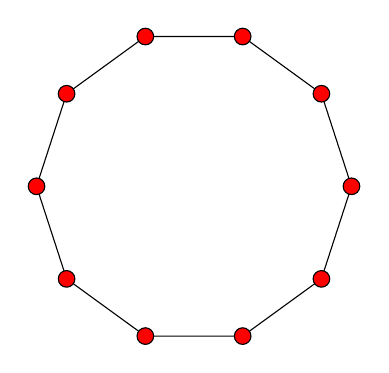
\begin{tikzpicture}
	\tikzstyle{every node}=[circle, draw, fill=red, inner sep=0pt, minimum width=6pt]
    \draw \foreach \x in {0,36,...,324}
    {
    	(\x:2) -- (\x+36:2)
    };
    \draw \foreach \x in {0,36,...,324}
    {
    	(\x:2) node {}
    };
\end{tikzpicture}\end{center}
\begin{center}
	\small Рис. 18. Граф $C_{10}$
\end{center}\end{paracol}

\begin{definition}
	Две вершины называют \emph{связанными}, если сущесвует хотя бы один путь, соединяющий их. Граф называют \emph{связным}, если любые две его вершины связаны. В противном случае он называется \emph{несвязным}.
\end{definition}

\begin{definition}
	Связный ациклический граф называют \emph{деревом}.
\end{definition}

	Дерево~---~самый многократно встречающийся граф в теории графов. 
	
\begin{definition}
	Граф $G$ называется \emph{цепью}, если он ацикличен и существует простой путь, который проходит через все вершины. Обозначается $P_n$.
\end{definition}

\begin{center}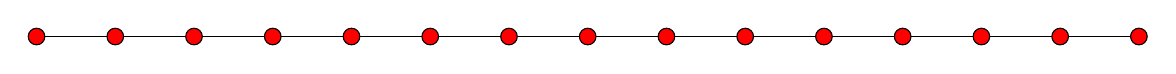
\begin{tikzpicture}
	\tikzstyle{every node}=[circle, draw, fill=red, inner sep=0pt, minimum width=6pt]
	
    \draw (0, 0) node {} -- (1, 0) node {} -- (2, 0) node {} -- (3, 0) node {} -- (4, 0) node {} -- (5, 0) node {} -- (6, 0) node {} -- (7, 0) node {} -- (8, 0) node {} -- (9, 0) node {} -- (10, 0) node {} -- (11, 0) node {} -- (12, 0) node {} -- (13, 0) node {} -- (14, 0) node {};
\end{tikzpicture}
\newline
\newline
	\small Рис. 19. Граф-цепь $P_14$
\end{center}

\begin{statement}
	Граф, в котором все вершины имеют степень либо $1$, либо $2$, состоит из циклов и цепочек.

\begin{proof}
	Рассмотрим висячую вершину $a_1$, допустим, что она соединена с вершиной $a_2$. Если $a_2$ тоже висячая, то эта часть графа закончилась и мы получили цепь длины $2$. Иначе есть смежная с $a_2$ вершина $a_3$. Повторяем для неё наши рассуждения. Таким образом, в силу конечности числа вершин на каком-то шаге у нас появится висячая вершина $a_k$ и закончится обход этой части графа.
	
	 Следовательно, предположим, что в какой-то части графа нет вершин со степенью, равной единице. Повторим алгоритм и в конце вершина $a_k$ обязательно будет соединена с вершиной $a_1$.
\end{proof}
\end{statement}

\begin{consequence}
	Если в графе все вершины имеют степень не больше двух, то рёбра графа можно раскрасить в $3$ цвета так, чтобы смежные рёбра были раскрашены в разные цвета. Кроме того, двух цветов хватит не для любого такого графа.
\end{consequence}

\mysubsection{Лемма о висячей вершине}

\begin{definition}
	Связный ациклический граф называют \emph{деревом}.
\end{definition}

	Мы не спроста повторили здесь определение, которое уже встречалось на предыдущей странице. На самом деле дерево можно задать очень разными, но в то же время эквивалентными формулировками. Мы будем придерживаться определения выше и выводить все свойства дерева именно из него.

\begin{definition}
	Вершина $a$ называется \emph{висячей}, если $deg(a) = 1$.
\end{definition}

\begin{lemma*}[о висячей вершине]
	В любом дереве с $n \geqslant 2$ вершинами найдутся хотя бы две висячие вершины.
	
\begin{proof}	
	 Во-первых, найдем одну висячую вершину. Для этого выберем произвольную вершину $a$ и рассмотрим какое-нибудь выходящее из этой вершины ребро. Пусть это ребро $\left\lbrace a, b \right\rbrace$. Если из вершины $b$ не выходит других ребер, то эта вершина~---~искомая. В противном случае отметим ребро $\left\lbrace a, b \right\rbrace$ и продолжим наш путь по любому неотмеченному ребру, выходящему из вершины $b$. И так далее. Заметим, что в строящемся таким образом пути ни одна вершина не встречается дважды, в противном случае получился бы цикл, а дерево ациклично. Поэтому при наличии неотмеченных ребер мы будем каждый раз переходить в неотмеченную вершину, а их конечное число. Следовательно, в конце концов наш путь закончится. Но закончится он может только в висячей вершине $с$ (см. рис. 20). 
	
	Во-вторых, повторим этот алгоритм, но в этот раз начнем уже с найденной нами висячей вершины $c$. Так как все вершины в нашем пути различны, то начало и конец нашего пути будут отличаться. Следовательно, мы нашли две висячие вершины.
\end{proof}
\end{lemma*}

\begin{center}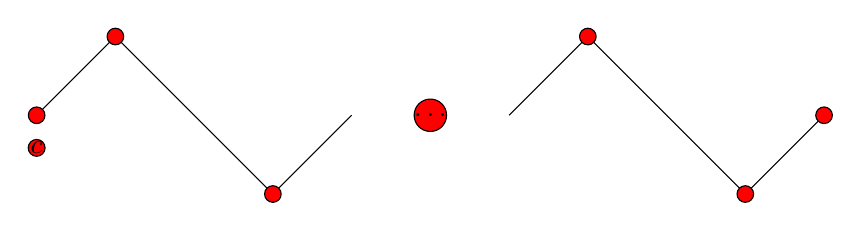
\begin{tikzpicture}
	\draw (5, 0) node []  {$\dots$};
	\draw (0, -0.3) node [below]  {$c$};

	\tikzstyle{every node}=[circle, draw, fill=red, inner sep=0pt, minimum width=6pt]
	
    \draw (0, 0) node {} -- (1, 1) node {} -- (3, -1) node {} -- (4, 0);
    \draw (6, 0) -- (7, 1) node {} -- (9, -1) node {} -- (10, 0) node {};
    
\end{tikzpicture}

	\small Рис. 20
\end{center}

\mysubsection{Свойства дерева. Остовы}

	Допустим, что перед нами стоит задача: найти подграф с минимальным количеством рёбер, который при этом был бы связным. Будем находить цикл в графе и удалять его. Легко проверить, что в таком случае граф не будет терять своей связности. В конце мы получим дерево, потому что конечный граф будет ациклическим.
	
	Так значит нам надо рассмоотреть все подграфы-деревья и выбрать то, в котором будет меньше рёбер, чтобы решить задачу? Нет, у них у всех будет оинаковое число рёбер, что мы докажем ниже.

\begin{statement}
	В любом дереве число вершин на единицу больше числа ребер, то есть $$|V| = |E| + 1.$$
	
\begin{proof}
	Воспользуемся методом математической индукции. Счётчиком у нас будет количество вершин в дереве.
	
	База индукции: при $|V| = 1$, очевидно, верна формула, так как ребер в этом дереве нет.
	
	Предположим, что при $|V| = k$ выполнена формула (заметим, что про саму структуру дерева мы ничего не говорим), и докажем, что при $|V| = k + 1$ она останется верной.
	
	Шаг индукции: так как мы имеем дело с деревом, то по У.Л.оВ.В. найдется висячая вершина в наешм графе. Тогда уберем эту вершину вместе с ребром, которое соединяет его с оставшимся графом. В остатке у нас будет всё еще дерево, при том оно будет иметь на одну вершину меньше, следовательно, для неё будет верна формула, то есть $$\left(|V| - 1\right) = \left(|E| - 1\right) + 1.$$
	Здесь за $V$ обозначено множество вершин исходного дерева, а за $E$~---~множество рёбер исходного дерева. Как видно, после раскрытия скобок мы получаем искомое выражение, что доказывает шаг индукции и завершает наше доказательство.
\end{proof}
\end{statement}

\begin{statement}
	При удалении ребра из дерева, оно теряет связность.
	
\begin{proof}
	Допустим противное, то есть при удалении ребра $e = {a, b}$ граф остался связным. Следовательно, вершины $a$ и $b$ в новом графе тоже связанны, а значит, есть путь $P$, который не проходит через $e$ и соединяет эти две вершины. Очевидно, что этот путь вместе с ребром $e$ будет порождать цикл в исходном графе. Противоречие.
\end{proof}
\end{statement}

\begin{consequence}
	Если при удалении ребра $e$ граф $G$ не теряет своей связности, то в нём есть цикл, проходящий через это ребро.
\end{consequence}

\begin{definition}
	Граф $O$ называется \emph{остовом} связного графа $G$, если $O$ имеет те же вершины, что и $G$, получается из $G$ удалением некоторых ребер и является деревом.
\end{definition}

\begin{statement}
	У всякого связного графа есть хотя бы одно остовное дерево.
\end{statement}

	Есть целый ряд задач, которые решаются сведением к более простой задачи. Например, некоторые задачи на графы можно решить, доказав что-нибудь для его остова.
	
	Чтобы получить остов, можно удалять рёбра, входящие в циклы или провести одну итерацию алгоритма в глубину. В чём состоит этот алгоритм?
	
	Сначала мы окрашиваем все вершины графа в белый цвет. Затем выбираем вершину $a$ и окрашиваем её в чёрный цвет. Если у $a$ есть смежная белая вершина $b$, то мы окрашиваем её и ребро $e = (a, b)$ в чёрный цвет и запускаем алгоритм для неё. Если все смежные с очередной вершиной уже окрашены в чёрный, то мы переходим на более высокий уровень рекурсии.
	
	Заметим, что в этом алгоритме мы использовали обозначение для ориентированного ребра, подразумевая под этим, что если мы имеем дело с орграфом, то алгоритм будет всё ещё иметь смысл. Но в этом случае он найдет не остовное дерево, а все вершины, в которые можно попасть из начальной вершины.

	Про этот алгоритм мы будем позже ещё много всего скажем, но уже в другой главе.
	


	

\mysubsection{Корневые деревья}

	

	Связный ациклический граф неспроста получил такое сочное название: его, действительно, можно представить в очень похожем на дерево виде. Для этого обозначим за корень какую-нибудь вершину дерева. Нарисуем корень. Далее все вершины графа, связанные с корнем, нарисуем ниже корня в ряд. Соединим их с корнем. Повторим эту операцию, считая нижние вершины за <<новые корни>>. Таким образом, мы получим граф, изоморфный нашему, очень похожий на перевернутый рисунок дерева.
	\newline
	\newline
	\tikzstyle{level 1}=[level distance=1.5cm, sibling distance=5.5cm]
	\tikzstyle{level 2}=[level distance=1.5cm, sibling distance=1.5cm]
	\tikzstyle{level 3}=[level distance=1.5cm, sibling distance=0.75cm]
	\tikz 
  	\node {Корень} 
    	child { node {Узел (1 уровень)}
    		child { node {$\dots$}
    			child { node {Лист}}}
    		child { node {$\dots$}
    			child { node {Лист}}}
    		child { node {$\dots$}
    			child { node {Лист}}}}
    	child { node {$\dots$} 
    		child { node {$\dots$}
    			child { node {Лист}}}
    		child { node {$\dots$}
    			child { node {Лист}}}
    		child { node {$\dots$}
    			child { node {Лист}}}}
    	child { node {Узел (1 уровень)}
    		child { node {$\dots$}
    			child { node {Лист}}}
    		child { node {$\dots$}
    			child { node {Лист}}}
    		child { node {$\dots$}
    			child { node {Лист}}}}
	;
\begin{center}
	\small Рис. 21. Общий вид дерева, с отмеченным корнем
\end{center}	

	Как вы можете заметить на рис. 21, вершина, за которую мы подвешиваем наше дерево, называется \emph{корнем} (root), промежуточные вершины называются \emph{узлами} (node), а все висячие вершины~---~\emph{листьями} (leaf). Кроме того, принято называть \emph{предками вершины $a$} все вершины, лежащие на пути из корня в вершину $a$; если вершина $b$~---~предок вершины $a$, то $a$~---~\emph{потомок вершины $b$}.
	
\mysubsection{Примеры}

\begin{example}
	На Марсе 200 кратеров, некоторые из которых соединены подземными тоннелями. Известно, что из любого кратера можно попасть в любой другой. Докажите, что вездеход может посетить все кратеры, пройдя не более 396 тоннелей.
	
	\emph{Доказательство.} Вспомним вид дерева, о котором мы говорили во втором параграфе, то есть тот, в котором есть корень, листья и промежуточные узлы. Заметим, что если в нём ровно один лист, то само дерево есть ни что иное, как цепочка. Но в ней очевидно можно начать с одного конца и дойти до другого, обойдя каждое ребро ровно один раз, то есть в сумме~---~99.
	
	Теперь разберёмся со случаем, когда у нас есть несколько листьев. Начнем наш путь в одном из них. Далее будем подниматься по уровням вверх. Если от очередного промежуточного узла отходит еще другая ветвь, то мы идем вниз по ней. Таким образом, мы обойдем все вершины и пройдем по всем ребрам, которые идут от предка вершины к ней самой не более двух раз. Кроме того, для начальной и конечной вершины мы знаем, что по соответствующему ребру мы пройдем ровно один раз. И у корня нет <<предшествующего>> ему ребра, так что мы пересечем ровно $(200 - 3) \cdot 2 + 2 \cdot 1 = 396$ тоннелей. ч.т.д.
\end{example}

\begin{example}
	Волейбольная сетка имеет вид прямоугольника $50 \times 600$ клеток. Какое наибольшее число веревок можно перерезать так, чтобы сетка не распалась на куски?
	
	\emph{Решение.} Построим граф, в котором вершинами будут узлы сетки, а рёбрами~---~веревочки. Остов~---~подграф с минимальным количеством рёбер. Поэтому нам надо убрать все ребра, кроме тех, которые лежат в выбранном нами остове. После нетрудных подсчётов получаем, что можно перерезать $30000$ веревочек.
\end{example}

\mysubsection{Дополнительные определения}

 В некоторых задачах также удобно будет пользоваться понятием дополнения графа. На самом деле дополнение к чему-либо можно встретить во многих областях математики, так что это определение полезно знать независимо оттого, будет ли читатель впоследствии его использовать в теории графов или нет.
	 
\begin{definition}
	\emph{Дополнением к графу $G\left(V, E\right)$} называется граф $\overline{G}$, в котором множество вершин совпадает с $V$, а рёбра получаются разностью рёбер полного графа и исходного, то есть $E' = (V \times V )\setminus E$.
\end{definition}

\begin{center}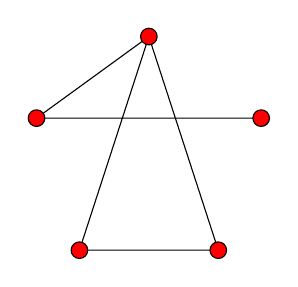
\begin{tikzpicture}
	\tikzstyle{every node}=[circle, draw, fill=red, inner sep=0pt, minimum width=6pt]
	
	\draw (18:1.5) -- (162:1.5) -- (90:1.5) -- (234:1.5) -- (306:1.5) -- (90:1.5);
    
    \draw \foreach \x in {18,90,...,306}
    {
    	(\x:1.5) node {}
    };
\end{tikzpicture}
\;\ \;\ \;\ \;\ \;\ \;\ \;\ \;\ \;\ \;\ \;\ \;\ \;\
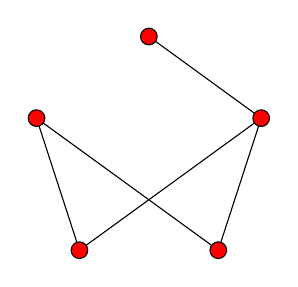
\begin{tikzpicture}
	\tikzstyle{every node}=[circle, draw, fill=red, inner sep=0pt, minimum width=6pt]
	
	\draw (306:1.5) -- (18:1.5) -- (90:1.5);
    \draw (306:1.5) -- (162:1.5) -- (234:1.5) -- (18:1.5);
    
    \draw \foreach \x in {18,90,...,306}
    {
    	(\x:1.5) node {}
    };
\end{tikzpicture}
\newline
\newline
	\small Рис. 22. Слева граф $G$, а справа его дополнение
\end{center}

	Чтобы получить из графа $G(V, E)$ граф $\overline{G}$ можно построить полный граф $K_n$, где $n = |V|$, и в нём убрать все рёбра, принадлежащие грау $G$.

\begin{definition}
	\emph{Лес}~---~упорядоченное множество деревьев.
\end{definition}

\begin{definition}
	\emph{Расстоянием $d(a, b)$ между вершинами $a$ и $b$} называется длина наименьшего пути, соединяющего их.
\end{definition}
	
	Заметим, что такой путь всегда простой. Кроме того, чтобы это понятие распространялось на несвязные графы, принято считать, что для несвязанных вершин $c$ и $e$ расстояние $d(c, e) = \infty$.

$ $
\newline
	В заключение подчеркнём важность доказанной леммы о висячей вершине, так как это не сильно затратное необходимое условие, с помощью которого можно мгновенно сказать, что граф не является деревом. Остов графа может помочь читателю вскрыть ни одну задачу.

\mysubsection{Задачи}

\begin{exersize}
	На каникулах братья Володя и Никита от скуки придумали следующую игру. У них на стене весела карта России с отмеченными на ней железными дорогами. За ход разрешалось взять маркер и <<перерезать>> одну из ж/д дорог, но только в том случае, если города, которые соединяет эта дорога не потеряют от этого сообщение между друг другом. Проигрывал тот, кто не мог больше сделать ход. Докажите, что, посмотрев на изначальную карту России, можно сказать еще до окончания игры, кто выиграет.
\end{exersize}

\begin{exersize}
	Сколько рёбер в дополнении дерева на $n$ вершинах?	
\end{exersize}	

\begin{exersize}
	Докажите, что граф является деревом тогда и только тогда, когда каждые две его вершины соединены ровно одним простым путем.
\end{exersize}	

\begin{exersize}
Докажите, что связный граф, у которого число рёбер на единицу меньше числа вершин, является деревом.
\end{exersize}

\begin{exersize}
	a) Ребра дерева окрашены в два цвета. Если в какой-то вершине сходятся ребра одного цвета, то можно их все перекрасить в другой цвет. Можно ли все дерево сделать одноцветным?
	
	b) Будем красить в два цвета не ребра, а вершины графа. Можно ли любое дерево раскрасить так, что любое ребро будет соединять вершины разных цветов?
	
	c) Докажите, что вершины графа можно раскрасить в два цвета тогда и только тогда, когда граф не содержит циклов нечетной длины.
\end{exersize}	

\begin{exersize}
	В течение предвыборной кампании каждый из 600 чиновников от партии <<Кедровое ядрышко>> жал руку ровно одному своему коллеге. Докажите, что после переизбрания президента можно на 200 государственных мест назначить чиновников из этой партии так, что среди выбранных чиновников никто никому не жал руку.
\end{exersize}	

\begin{exersize}
	В стране 45 городов, некоторые из них соединены авиалиниями, принадлежащими трём авиакомпаниям. Известно, что даже если любая из авиакомпаний прекратит полёты, можно будет добраться из любого города в любой другой (возможно, с пересадками), пользуясь рейсами оставшихся двух компаний. Какое наименьшее число авиалиний может быть в стране?
\end{exersize}	

\begin{exersize}
	Степенная последовательность дерева имеет вид $7, 6, 5, 4, 3, 2, 1, \dots, 1$. Сколько рёбер в этом дереве?
\end{exersize}	

\begin{exersize}
	Пусть в дереве четное количество рёбер. Докажите, что в таком дереве обязательно найдется хотя бы одна вершина чётной степени.
\end{exersize}	

\begin{exersize}
	Докажите, что в любом связном графе можно удалить вершину вместе со всеми выходящим ребрами так, чтобы он остался связным.
\end{exersize}	

\begin{exersize}
	Дано дерево с $n \geqslant 2$ вершинами. В каждую вершину поставили по действительному числу $x_1, x_2, \dots, x_n$. Далее на каждом ребре записали произведение чисел в концевых вершинах. Сумма всех чисел на рёбрах получилась равной $S$. Докажите, что имеет место следующее неравенство $$\sqrt{n-1} (x_1^2 + x_2^2 + \dots + x_n^2) \geqslant 2S.$$
\end{exersize}	

\begin{exersize}
	Докажите, что нельзя так раскрасить кубик с гранью в одну клетку в чёрный и белый цвета, чтобы его можно было прокатить по доске и он побывал на каждой клетке единожды и каждый раз соприкасающаяся с доской грань кубика и клетка, на которой он стоит, были одного цвета.
\end{exersize}	